As it has been said before, part of SEN12MS-CR-TS \cite{sen12mscrts} will be included in the original dataset SEN12MS-CR \cite{sen12mscr}. However, since there is no paired images in the dataset, some adjustments should be carried out.
Overall, there is a 55 \% of cloudy images. Hence, inherently, a pairing of the dataset could be done just by choosing the 45 \% cloudless images and the ones left. However, a bias would be produced since we would be inject 14 \% pairings of the same patch.
\begin{figure}[H]
	\centering
	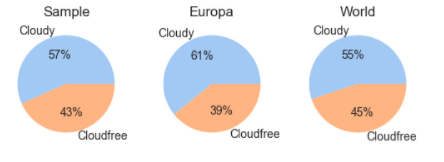
\includegraphics[width=8cm]{imgs/eda/merge/cloudies}
	\caption{Cloudy images percentage in SEN12MS-CR-TS.}
	\label{fig:eda-merge-classifcation}
\end{figure}
To know better which kind of pairing I was dealing with, a visualization of a sample of 10 patches from any time interval was done to check have a simple overview of a patch given the 30 intervals, as it is depicted in figure \ref{fig:eda-merge-patch-xploration}.
\\
\\
To classify which images are cloudy and cloudless, it has been defined a limit of the mean of the cloud percentage area in \cite{sen12mscr} from the former exploratory data analysis. This is shown in figure \ref{fig:eda-merge-classifcation}, given the patch shown in figure \ref{fig:eda-merge-patch-xploration}.
\begin{figure}[H]
	\centering
	\begin{adjustwidth}{-2cm}{}
	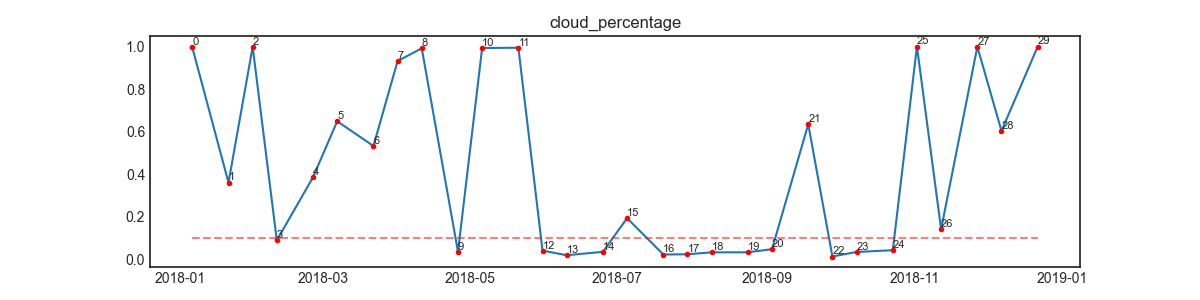
\includegraphics[width=18cm]{imgs/eda/merge/cloud-percentages-patch-plot}
	\end{adjustwidth}
	\caption{Patch exploration in all intervals.}
	\label{fig:eda-merge-classifcation}
\end{figure}
It is notable to mention how similar are the classification from the patch shown and the cloud percentage distribution of the entire dataset, as it is depicted in \ref{fig:eda-merge-patch-distribution}. This is due to the range of image capture of each time interval, since no time instant\footnote{Time instant and time interval are used indistinctively in that case.} from any patch is more than 6 days away from any other patch given the time instant id. 
\begin{figure}[H]
	\centering
	\begin{adjustwidth}{-2cm}{}
		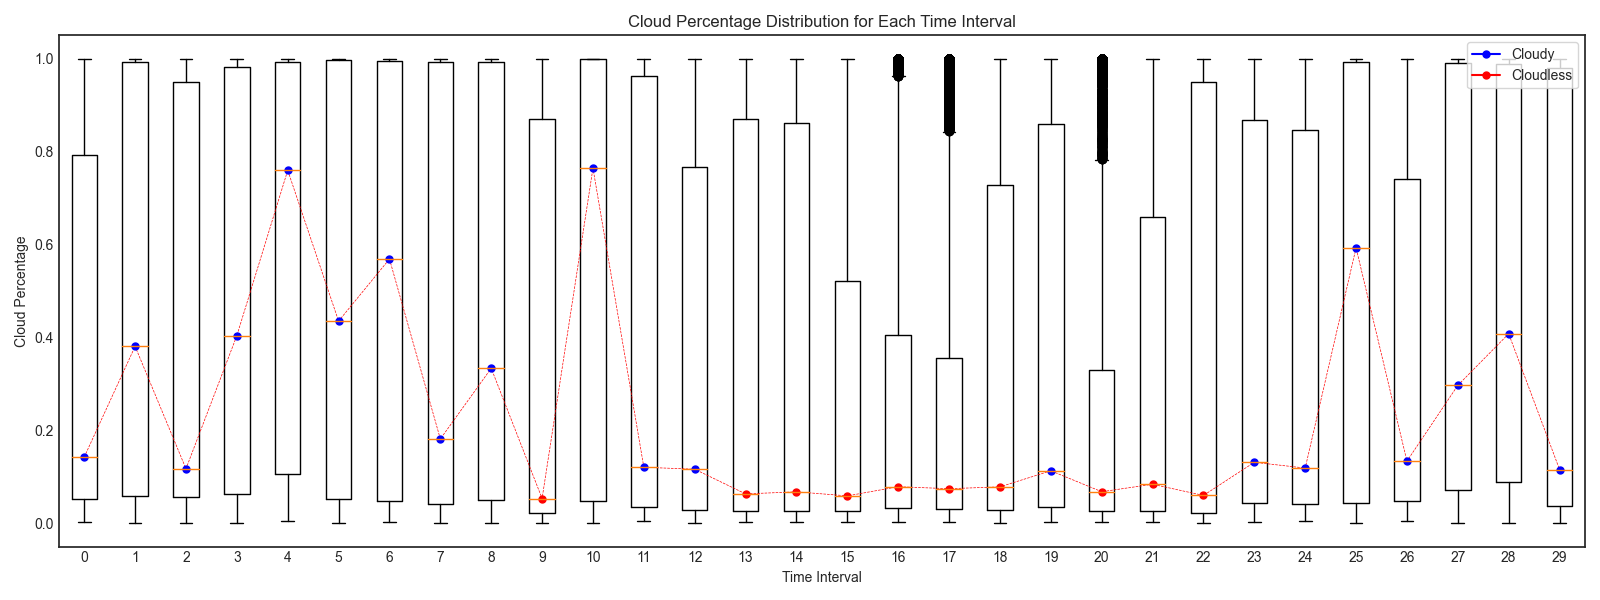
\includegraphics[width=18cm]{imgs/eda/merge/cloud-percentage-each-time-interval}
	\end{adjustwidth}
	\caption{Cloud percentage distribution in all intervals and its possible classification given the median.}
	\label{fig:eda-merge-patch-distribution}
\end{figure}
Additionally, each band and index has been compared to the cloud percentage of the given time instance to check if some anomalies were found. In fact, it has been discovered that when an image got blurred, the indices \texttt{MSI}, \texttt{NDWI} and \texttt{NDSI} are more affected than the others. Actualy, all these indices are created by bandwidths B3 and B8 and they are about the presence of moisture, water, snow respectively. Therefore, the anomaly found in the B3 and B8 can be just depicting a storm than showing a discordancy between the output of the cloud model and the image itself. This phenomenon has also been aligned with the behaviour of SEN12MS-CR, although was not presence in all the imagery.
\begin{figure}[H]
	\centering
	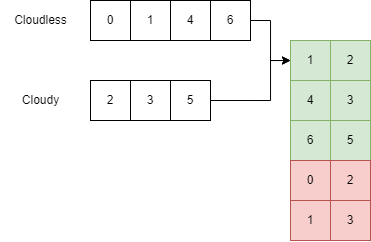
\includegraphics[width=8cm]{imgs/eda/merge/matching}
	\caption{Pairing algorithm.}
	\label{fig:eda-merge-matching}
\end{figure}
Once analysed the dataset and found that they have more or less the same qualities and characteristics from base dataset, it has been developed an algorithm to pair the images. Considering that each patch has two vectors, one at a time when the images are cloudy and another when they are cloud-free, a resultant vector is created from the possible pairs ordered by the minimum distance of these moments in time. In this way, the modification of the terrain will be minimal. Moreover, instead of doing of every vector, it has been split the patch into the seasons, so the resulting number of pairings found is \texttt{30097}. Hence, the data grows up to $(101613 + 30097) = 131710$ pairings, increasing a $29.16 \%$ more. Nevertheless, since it is added some bias to the dataset, a comparison between models trained with only SEN12MS-CR and with the data augmentation should be carried out.
